\clearpage

\section{Resample}

\begin{tcolorbox}	
	\begin{tabular}{p{2.75cm} p{0.2cm} p{10.5cm}} 	
		\textbf{Header File}   &:& resample$\_*$.h \\
		\textbf{Source File}   &:& resample$\_*$.cpp \\
        \textbf{Version}       &:& 20180423 (Celestino Martins) \\
        					   &:& 20190509 (Daniel Pereira)
	\end{tabular}
\end{tcolorbox}

This block simulates the resampling of a signal. It receives one input signal and outputs a signal with the sampling rate defined by sampling rate, which is externally configured.

\subsection*{Input Parameters}

\begin{table}[h]
	\centering
	\begin{tabular}{|c|c|c|c|cccc}
		\cline{1-4}
		\textbf{Parameter} & \textbf{Type} & \textbf{Values} &   \textbf{Default}& \\ \cline{1-4}
		rFactor           & double & any & $inf$ \\ \cline{1-4}
		samplingPeriod    & double & any & $0.0$ \\ \cline{1-4}	
        symbolPeriod      & double & any & $1.5$ \\ \cline{1-4}	
	\end{tabular}
	\caption{Resample input parameters}
	\label{table:resample_in_par}
\end{table}


\subsection*{Methods}

Resample() {};
Resample(vector$<$Signal *$>$ \&InputSig, vector$<$Signal *$>$ \&OutputSig) :Block(InputSig, OutputSig)\{\};

void initialize(void);
bool runBlock(void);

void setSamplingPeriod(double sPeriod) { samplingPeriod = sPeriod; }
void setSymbolPeriod(double sPeriod) { symbolPeriod = sPeriod; }

void setOutRateFactor(double OUTsRate) { rFactor = OUTsRate; }
double getOutRateFactor() { return rFactor; }

\subsection*{Functional description}

This block can performs the signal resample according to the defined input parameter \textit{rFactor}. It resamples the input signal at rFactor times the original sample rate.

Firstly, the parameter \textit{nBits} is checked and if it is greater than 1 it is performed a linear interpolation, increasing the input signal original sample rate to rFactor times.


\pagebreak
\subsection*{Input Signals}

\subparagraph*{Number:} 1

\subsection*{Output Signals}

\subparagraph*{Number:} 1

\subparagraph*{Type:} Electrical complex signal

\subsection*{Examples}

\subsection*{Version 20190506}

Version 20190509 adds the option to use FIR interpolation using a multiphase interpolation filter similar to the one presented in Figure~\ref{fig:FILTER}.

\begin{figure}[h]
\centering
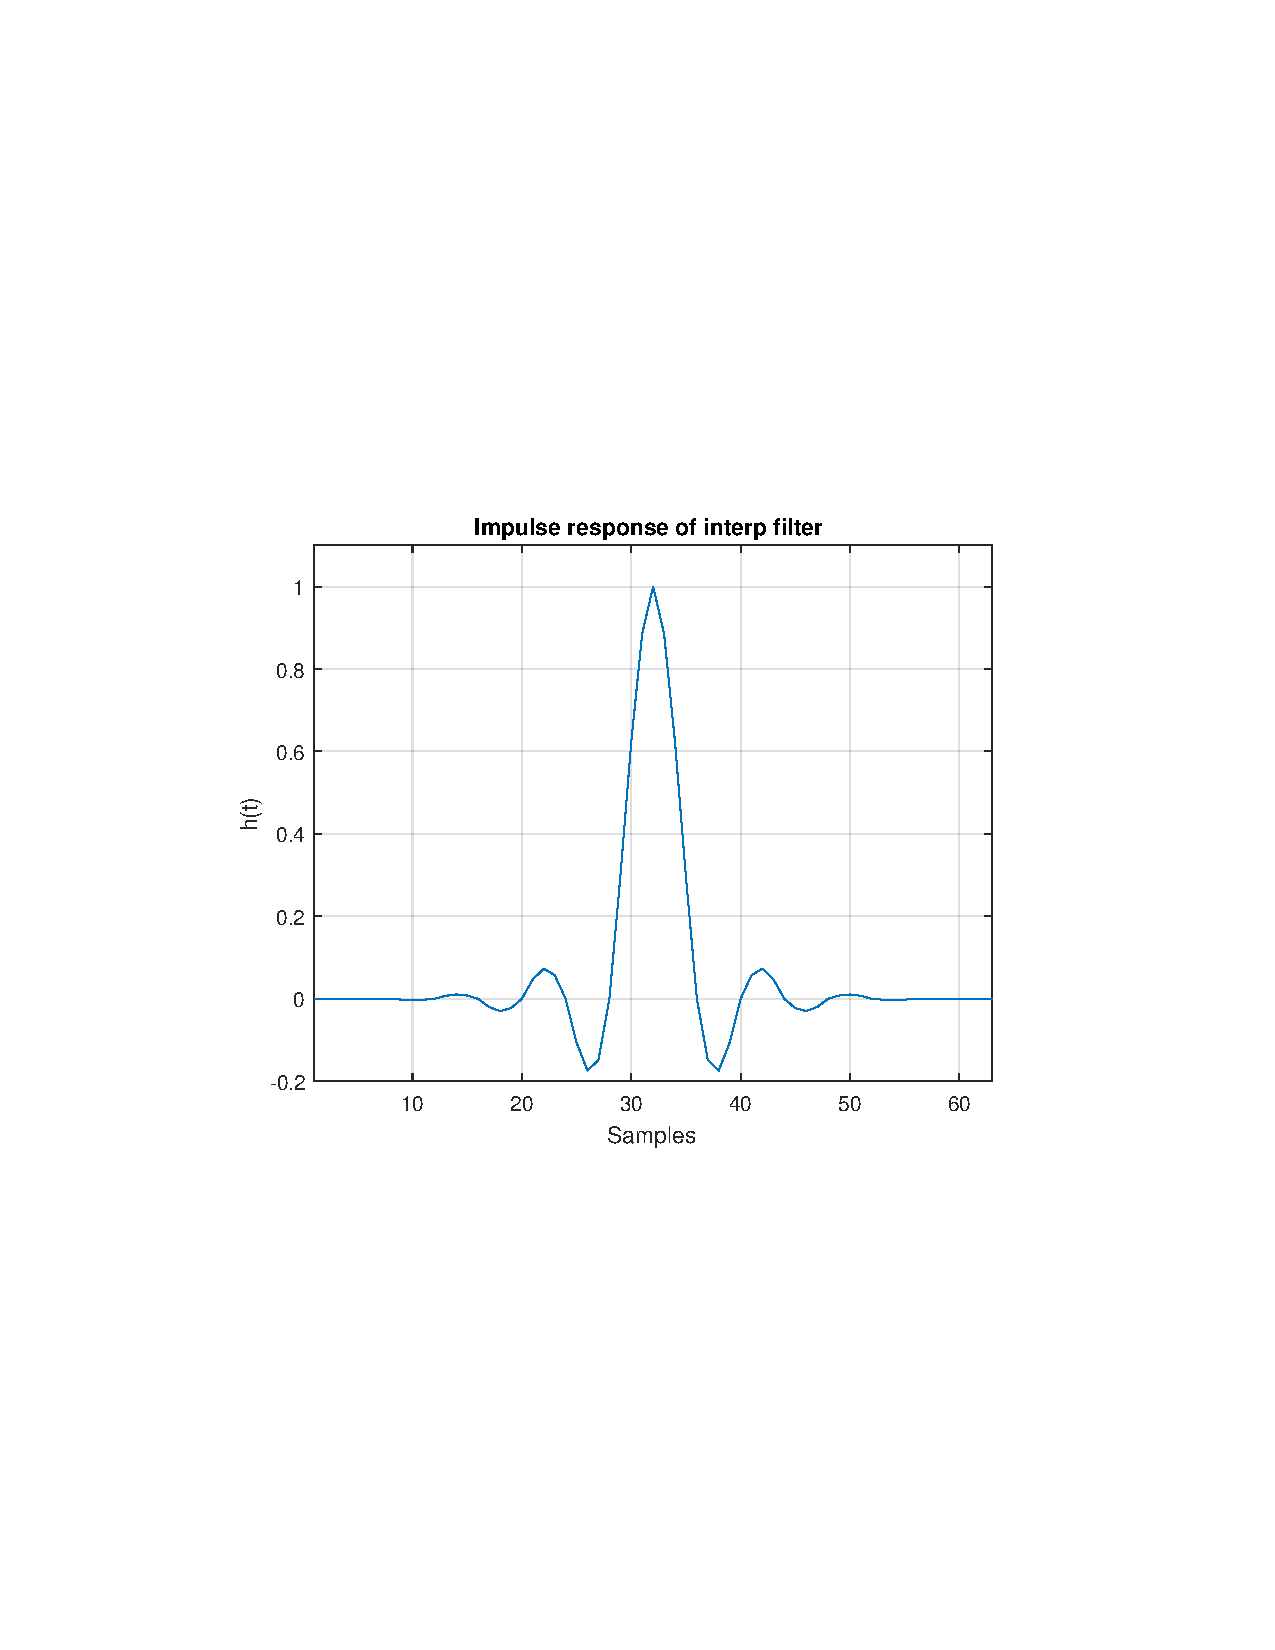
\includegraphics[trim={7cm 8cm 7cm 8cm},width=.3\linewidth]{./lib/resample/figures/FILTER}
\caption{Impulse response of a 4$\times$ upsampling filter using 16 taps.}
\label{fig:FILTER}
\end{figure}	

\begin{itemize}
  \item \textbf{Input Parameters}
  \begin{table}[H]
    \centering
    \begin{tabular}{|l|l| m{4cm}|l|}
    \hline
    Name & Type & Values & Default Value \\ \hline
    mode & UpSamplingMode & LinearInterpolation, FIRFilterInterpolation & LinearInterpolation \\ \hline
    numberOfTaps & int & any & 8 \\ \hline
    \end{tabular}
  \end{table}

  \item \textbf{Methods}
  \begin{itemize}
    \item void setNumberOfTaps(int nTaps) \{ numberOfTaps = nTaps; \}
    \item void setMode(UpSamplingMode m) \\ \{ mode = m; \}
  \end{itemize}
\end{itemize}

\subsection*{Sugestions for future improvement}


